\section{Filtro pasabajos}

Se pidió aplicar a un filtro RC de frecuencia de corte $f_{0}=64\,(kHz)$
una onda cuadrada de $10\,V_{pp}$ con frecuencia de $f=32\,(kHz)$
. Los resultados obtenidos empiricamente fueron los que se muestran
en las figuras \ref{2_1} y \ref{2_4}. A su vez, se calculo la transferecia
del circuito idealmente resultando ser:

\begin{equation}
H(s)=\frac{1}{1+sRC}\label{eq:2_4}
\end{equation}

Si simulamos la transferencia del circuito en LTSpice, el resultado
es el que se ve en las figuras \ref{2_4} y \ref{2_5}.

\begin{figure}[h]
\begin{centering}
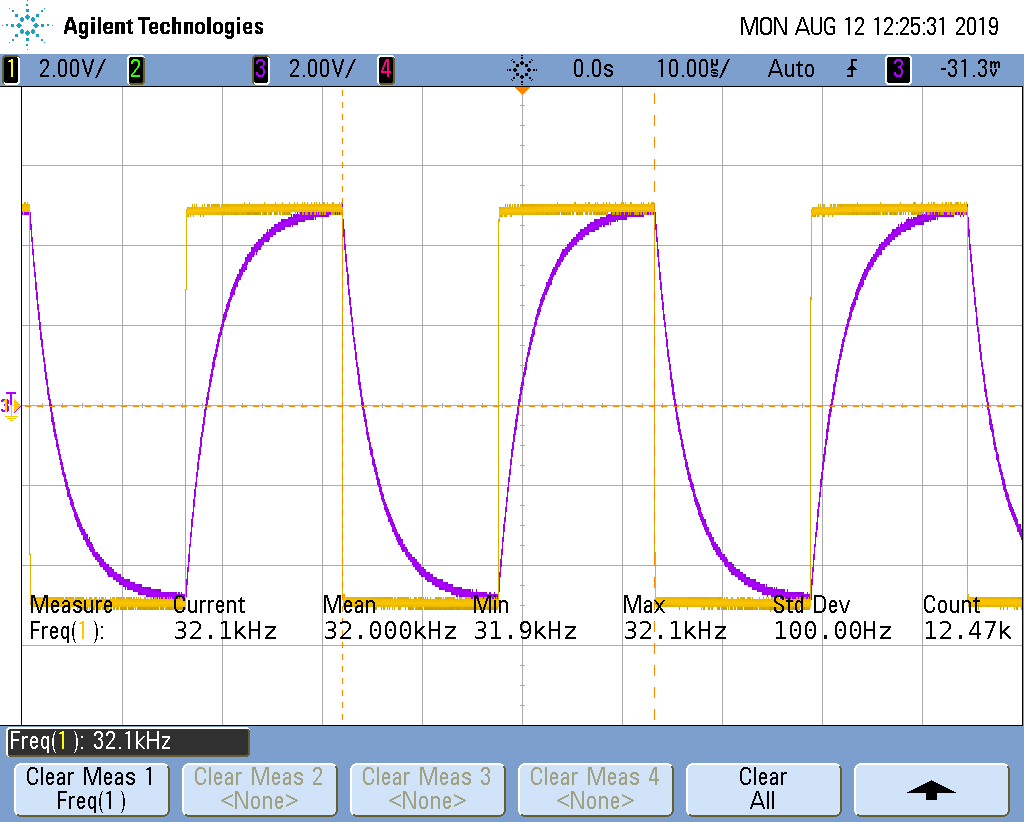
\includegraphics[scale=0.4]{resources2/scope_0}
\par\end{centering}
\caption{Resultados}
\label{2_1}
\end{figure}

\begin{figure}[h]
\begin{centering}
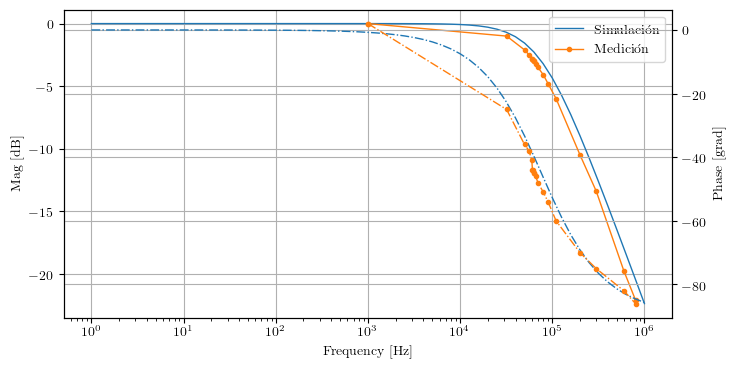
\includegraphics[scale=0.65]{resources2/MedyPost}
\par\end{centering}
\caption{Simulacion LTSpice y Mediciones}
\label{2_4}

\end{figure}

\begin{figure}[h]
\begin{centering}
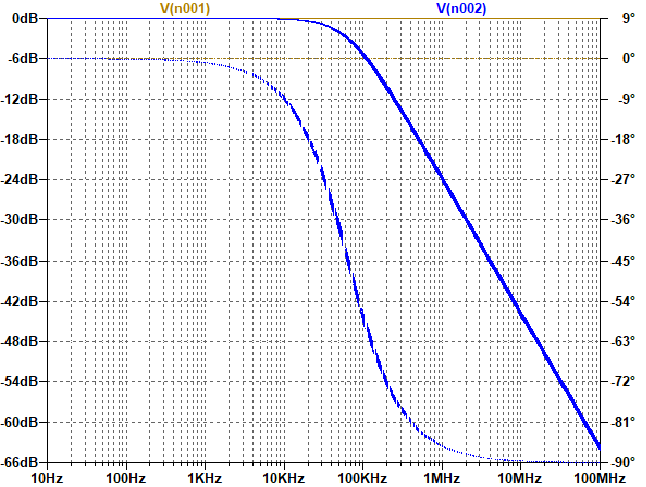
\includegraphics[scale=0.5]{resources2/montecarlo}
\par\end{centering}
\caption{Análisis montecarlo}
\label{2_5}
\end{figure}

\subsection{Calculo de armónicos}

Si queremos ver como reacciona el circuito a una señal cuadrada, debemos
calcular primero como afecta nuestro circuito a la onda de entrada.
Como sabemos que la onda es una cuadrada, haciendo su descomposición
de suma de señales trigonometricas, los coeficientes de Fourier resultan
ser:

\[
a_{0}=0
\]

\[
a_{n}=0
\]

\[
b_{2n-1}=\frac{20}{(2n-1)\pi}
\]

\[
b_{2n}=0
\]

Por lo tanto, la onda cuadrada se puede expresar en el espacio temporal
como se ve en la expresión \ref{eq:2_1}. Sin embargo, podemos ver,
por temas de idealizacion, que una señal cuadrada ideal, se puede
aproximar por una suma de términos finitos de senoidales, por lo tanto,
si aproximamos la cuadrada con 10 terminos, podemos ver como la aproximacion
van quedando mas parecidas, esto se muestra en la figura \ref{2_2}.
A medida que agreguemos mas términos a nuestra suma, menos sera la
diferencia con una onda cuadrada ideal. No obstante, hay que tener
en cuenta que, como fue visto en Matemática V, al tener una discontinuidad
no evitable cada $\frac{T}{2}$, siendo \emph{T} el período de la
señal, se generaran sobrepicos en los puntos de discontinuidad. por
ende, si llamamos \emph{x(t)} a la función cuadrada ideal e \emph{y(t)}
a su aproximación por senoides, \emph{x(t)} será igual a \emph{y(t)
}en todos los numeros reales exceptuando los puntos de discontinuidad.
Esto quiere decir, que es posible que al trabajar con ondas cuadradas,
se encuentren sobrepicos.

\begin{equation}
x(t)\sim\sum_{n=1}^{\infty}\frac{20}{(2n-1)\pi}sin\left(2\pi(2n-1)f_{0}t\right)\label{eq:2_1}
\end{equation}

\begin{figure}[h]
\begin{centering}
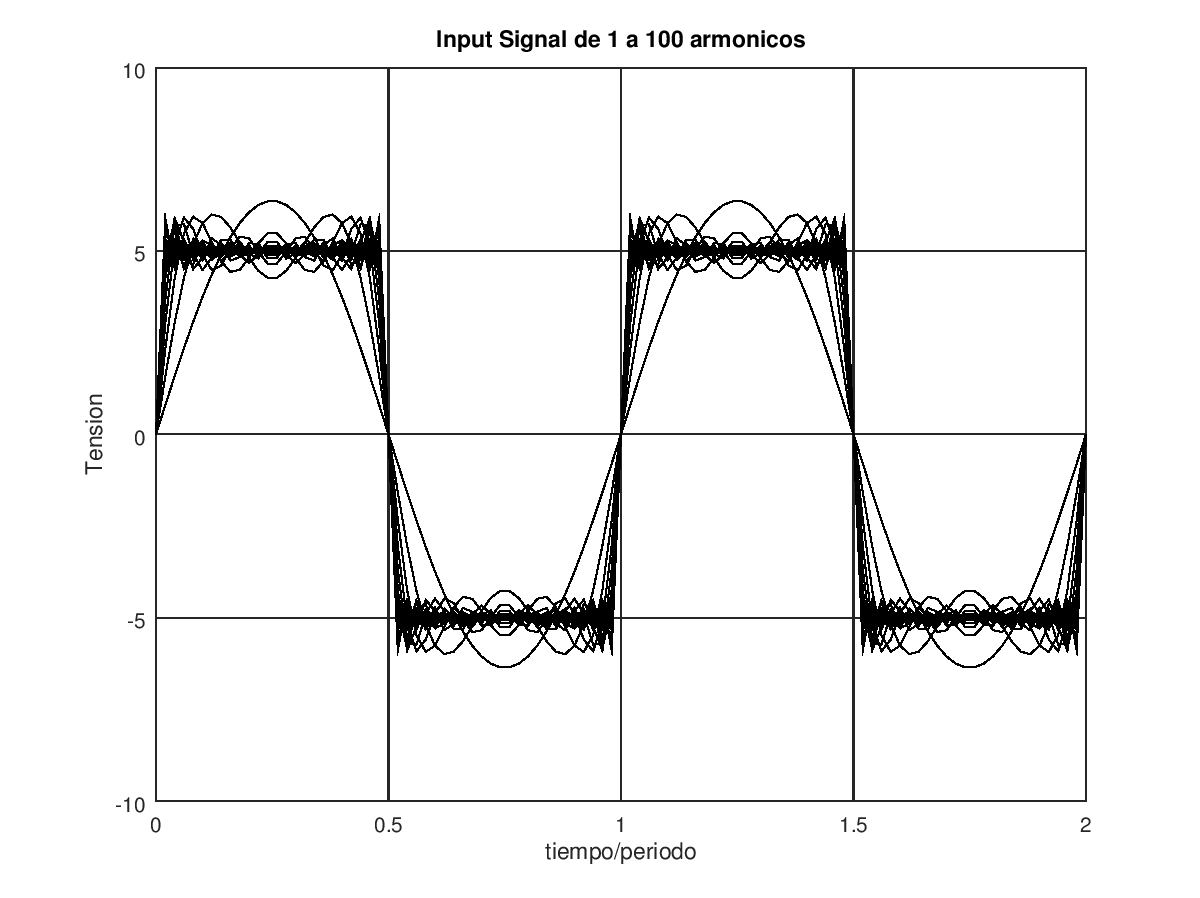
\includegraphics[scale=0.35]{resources2/Square}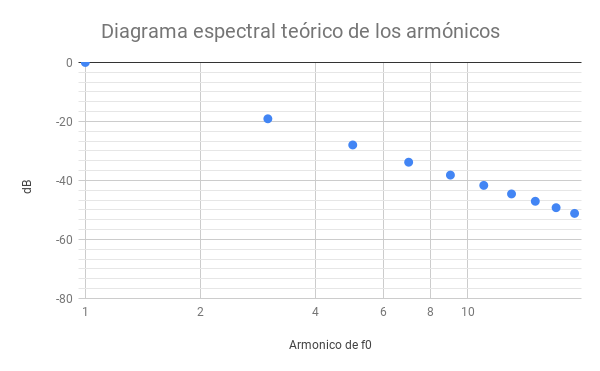
\includegraphics[scale=0.35]{resources2/DiagEspcTeo}
\par\end{centering}
\caption{Representación de onda cuadrada mediante suma de senoidales y su diagrama
espectral teórico}
\label{2_2}
\end{figure}

\begin{figure}[h]
\begin{centering}
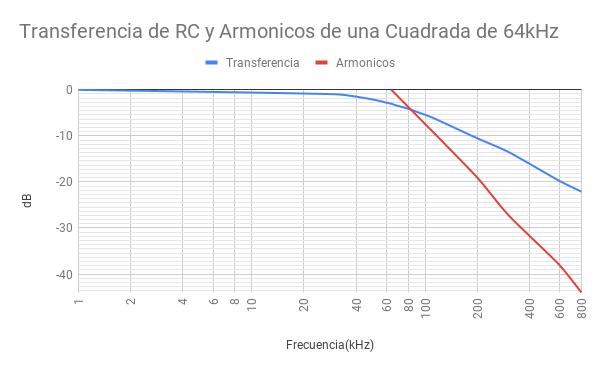
\includegraphics[scale=0.4]{resources2/Med_Arm}
\par\end{centering}
\caption{Transferencia superpuesta con los armonicos(los ptos de los armonicos
están unidos por lineas)}

\end{figure}

Debido a que la entrada es una función continua a trozos de período
\emph{T, }entonces:

\[
y(t)\sim\sum_{n=1}^{\infty}\left|b_{2n-1}\right|\left|H\left((2n-1)f_{0}\right)\right|cos\left[2\pi(2n-1)f_{0}t+\phi((2n-1)f_{0})+\theta_{2n-1}\right]
\]

\begin{equation}
b_{2n-1}=\left|b_{2n-1}\right|e^{i\theta_{2n-1}}\label{eq:3}
\end{equation}

\[
H(f)=\left|H(f)\right|e^{i\phi(f)}
\]

A su vez;

\begin{equation}
H(f)=\frac{1}{1+i2\pi fRC}\label{eq:2}
\end{equation}

Por lo tanto, haciendo calculos de las ecuaciones \ref{eq:3} y \ref{eq:2},
concluimos que:

\[
\phi(f)=-arctg(2\pi fRC)
\]

\[
H(f)=\frac{1}{\sqrt{(2\pi fRC)^{2}+1}}
\]

\[
\theta_{n}=0
\]

Finalmente, podemos escribir la salida como la ecuacion \ref{eq:2_3}
y graficamente se ve como la figura \ref{2_3}.

\begin{equation}
y(t)\sim\sum_{n=1}^{\infty}\frac{20}{(2n-1)\pi\sqrt{\left(2\pi(2n-1)f_{0}RC\right)^{2}+1}}cos\left(2\pi(2n-1)f_{0}t-arctg\left(2\pi(2n-1)f_{0}RC\right)+\frac{\pi}{2}\right)\label{eq:2_3}
\end{equation}

Teniendo en cuenta que $f_{0}=\frac{1}{2\pi RC}$ , y llamando \emph{k=2n-1,
}entonces

\[
y(t)\sim\sum_{k\,impares}\frac{20}{k\pi\sqrt{k^{2}+1}}cos\left(2\pi kf_{0}t-arctg\left(k\right)+\frac{\pi}{2}\right)
\]

\begin{figure}[h]
\begin{centering}
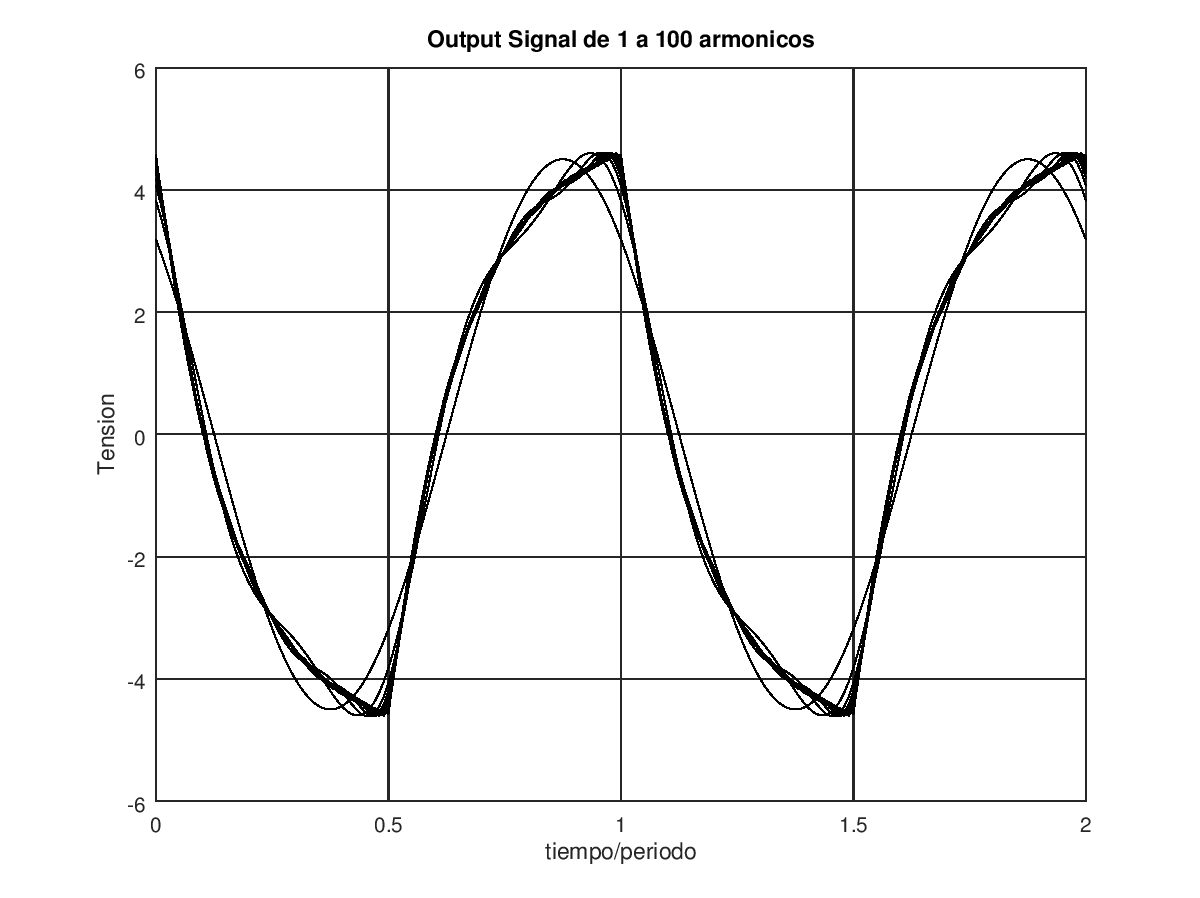
\includegraphics[scale=0.5]{resources2/out_calc}
\par\end{centering}
\caption{Salida del RC en armónicos}
\label{2_3}
\end{figure}

\subsection{Circuito como Integrador}

Como ya sabemos, un circuito integrador es aquel que cumple que su
funcion transferencia sea $H(s)=\frac{1}{s}$, como vemos en la ecuacion
\ref{eq:2_4}, nuestro circuito no posee esa transferencia, sin embargo,
si procuramos movernos en un intervalo donde \emph{sRC }sea lo suficientemente
grande comparado con 1, podremos aproximar a una funcion transferecia
integradora. Es decir;

\[
Si\,\,sRC\ggg1\Longrightarrow H(s)=\frac{1}{1+sRC}\approx\frac{1}{RC}\frac{1}{s}
\]

Por ende, si cambiamos al espacio de frecuencias, procurando que $2\pi fRC\ggg1$
podemos obtener la transferencia de un circuito integrador. En particular,
para $R=3.68(k\Omega)\,y\,C=560(pF)$ debemos concluir que para una
frecuiencia $f_{a}\ggg63(kHz)$, nuestro circuito se comportará como
un integrador.

En particular, si tenemos una frecuencia $f_{i}=300(kHz)$, $2\pi f_{a}RC\gg1$,con
lo cual podemos aproximar el denominado de la transferencia y usar
nuestro circuito como integrador, como se puede observar en la figura
\ref{2_6}.

\begin{figure}[h]
\begin{centering}
\includegraphics[scale=0.4]{resources2/300k}
\par\end{centering}
\caption{Circuito como integrador a 300 (kHz)}
\label{2_6}

\end{figure}

\begin{figure}[h]
\begin{centering}
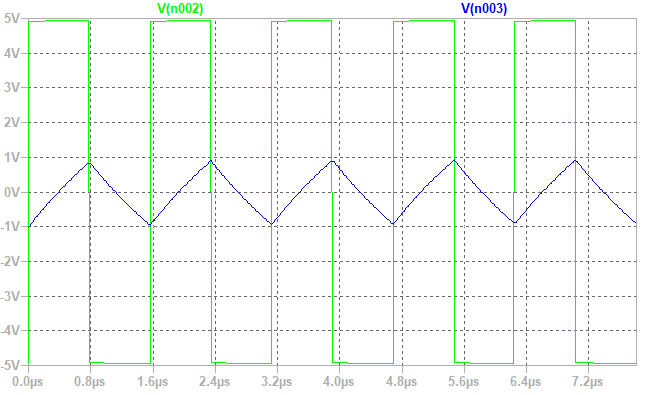
\includegraphics[scale=0.6]{resources2/sim}
\par\end{centering}
\caption{Simulacion del circuito a 300 (kHz)}

\end{figure}

\begin{figure}[h]
\begin{centering}
\includegraphics[scale=0.4]{resources2/640}
\par\end{centering}
\caption{Circuito andando a 640(Hz)}

\end{figure}